\subsection{进一步近似}
更令人感兴趣的是鞍点方程(\ref{H[w]相对w(r)的变化})的非平凡解。通常需要通过数值的方法来得到这种平均场解的精确描述。数值方法的讨论推迟到第5.3节;在这里,我们考虑进一步的分析近似,使不平凡的鞍点方程易于处理。这些近似基于第3.4节中提出的方法,用于估计外部势场中单链的统计特性。
\subsubsection{弱非均匀展开-RPA}
可以与平均场近似一起应用的一种重要的近似类型是弱非均匀展开。在方程(\ref{H[w]相对w(r)的变化})的解几乎是一致的情况下,我们可以用方程(3.113)类比得出
\begin{equation}\label{5.23}
w^*(\br)=w_0+\omega^*(\br)
\end{equation}
其中$w_0\equiv(1/V)\int w^*(\br)\mathrm{d}\br$是体积平均的平均场势场,假设偏差$\omega^*(\br)$与$w_0$相比在任何地方都很小,可以通过3.4.1节的过程来推导弱非均匀展开。这种展开在聚合物文献中通常称为随机相近似,或RPA(de Gennes,1969;de Gennes,1979)。我们用正则模型A来说明它。

正则模型A的鞍点方程由方程(\ref{5.16})中给出。用方程(\ref{5.23})代替方程(\ref{5.16})中$w^*(\br)$并应用方程(3.134)和(4.75)导出以下扩展:
\begin{equation}\label{5.24}
u_0^{-1}\omega^*(\br)+\rho_0N\int g_D(\left|\br-\br'\right|)\omega^*(\br')\mathrm{d}\br'+O((\omega^*)^2)=0
\end{equation}
其中方程(\ref{5.17})用于消去齐次项,$g_D(r)$是方程(3.133)的Debye函数。方程(\ref{5.24})的唯一解是$\omega^*(\br)=0$,这与我们之前的结论一致,即正则模型A在整体区域或具有周期性边界条件单元的唯一鞍点是平凡解$w^*(\br)=w_0$。\\
证明:由$w^*(\br)=w_0+\omega^*(\br)$和$\tilde{\rho}(\br;[iw])=n\rho(\br;[iw])$以及
\begin{equation*}
\rho(r;[w])\sim\rho_0[1-\epsilon_aN\int g_D(|\br-\br'|)]w(\br')\mathrm{d}\br'+O(\epsilon_a^2)]
\end{equation*}
所以
\begin{equation*}
\frac{1}{u_0}w^*(\br)+i\tilde{\rho}(\br;[iw^*])=0
\end{equation*}
\begin{equation*}
\frac{1}{u_0}[w_0+\omega^*(\br)]+i\rho_0+\rho_0N\int g_D(|\br-\br'|)]\omega(\br')\mathrm{d}\br'+O((\omega)^2)=0
\end{equation*}
\begin{equation*}
\frac{1}{u_0}w_0+\frac{1}{u_0}\omega^*(\br)+i\rho_0+\rho_0N\int g_D(|\br-\br'|)]\omega(\br')\mathrm{d}\br'+O((\omega)^2)=0
\end{equation*}
\begin{equation*}
\frac{1}{u_0}\omega^*(\br)+\rho_0N\int g_D(|\br-\br'|)]\omega(\br')\mathrm{d}\br'+O((\omega)^2)=0
\end{equation*}
RPA展开还可用来观察密度函数$F[\rho]$的形式,这是第4.10节DFT形式的核心,在平均场近似中,正则模型A的方程(4.207)简化为
\begin{equation}\label{5.25}
\rho(\br)\approx\tilde{\rho}(\br;[iw^*+J])
\end{equation}
我们用$\rho(\br)$简写代替$\left\langle\hat{\rho}(\br)\right\rangle_J$。该等式确定了由任意外部势场$J(\br)$产生的平均段密度$\rho(\br)$。此外,在平均场近似中,方程(4.205)的配分函数简化为$\calZ_C[J]\approx\calZ_0\exp(-H[w^*,J])$,在这两个表达式中,鞍点$w^*(\br)$由下式确定
\begin{equation}\label{5.26}
\frac{\delta H[w,J]}{\delta w(\br)}\bigg|_{w=w^*}=u_0^{-1}w^*(\br)+i\tilde{\rho}(\br;[iw^*+J])=0
\end{equation}
通过选择振幅较弱的$J$并且具有消失的体积平均值,即$(1/V)\int J(\br)\mathrm{d}\br=0$,方程(\ref{5.26})的右端可以类似于方程(\ref{5.24})的RPA展开得出。关于$J$的一阶展开式为:
\begin{equation}
\begin{aligned}
\int[u_0^{-1}\delta(\br-\br')&+\rho_0Ng_D(\left|\br-\br'\right|)]\omega^*(\br')\mathrm{d}\br'\\
&=i\rho_0N\int g_D(\left|\br-\br'\right|)J(\br')+O(J^2)
\end{aligned}
\end{equation}
该结果的傅里叶变换产生以下与$\omega^*$和$J$相关的公式:
\begin{equation}\label{5.28}
\hat{\omega}^*(\bk)=\frac{iu_0\rho_0N\hat{g}_D(x)}{1+u_0\rho_0N\hat{g}_D(x)}\hat{J}(\bk)+O(J^2)
\end{equation}
其中$x=k^2R_g^2$是无量纲的平方波数,其具有未受扰动的回旋半径的平方$R_g^2=Nb^2/6$。\\
证明:
\begin{equation*}
\frac{1}{u_0}w^*(\br)+i\tilde{\rho}(\br;[iw^*+J])=0
\end{equation*}
\begin{equation*}
\begin{aligned}
\frac{1}{u_0}\omega^*(\br)&+\rho_0N\int g_D(|\br-\br'|)]\omega^*(\br')\mathrm{d}\br'\\
&=i\rho_0N\int g_D(|\br-\br'|)]J(\br')\mathrm{d}\br'+O(J^2)
\end{aligned}
\end{equation*}
由$f(r)=\int\delta(r-r')f(r')\mathrm{d}r'$得:
\begin{equation*}
\begin{aligned}
\int[u_0^{-1}\delta(\br-\br')&+\rho_0Ng_D(\left|\br-\br'\right|)]\omega^*(\br')\mathrm{d}\br'\\
&=i\rho_0N\int g_D(\left|\br-\br'\right|)J(\br')\mathrm{d}\br'+O(J^2)
\end{aligned}
\end{equation*}
傅里叶变换:
\begin{equation*}
\begin{aligned}
\text{左边}=&\frac{1}{u_0}\omega^*(\br)+\rho_0N\int g_D(|\br-\br'|)\omega^*(\br')\mathrm{d}\br'\\
=&\frac{1}{u_0}\int e^{-i\bk\br}\omega^*(\br)\mathrm{d}\br+\rho_0N\int e^{-i\bk\br}\mathrm{d}\br\int g_D(|\br-\br'|)\omega^*(\br')\mathrm{d}\br'\\
=&\frac{1}{u_0}\int e^{-i\bk\br}\omega^*(\br)\mathrm{d}\br+\rho_0N\int e^{-i\bk(\br-\br')}g_D(|\br-\br'|)\mathrm{d}\br\int e^{-i\bk\br'}\omega^*(\br')\mathrm{d}\br'\\
=&\frac{1}{u_0}\hat{\omega}^*(\bk)+\rho_0N\hat{g}_D(x)\hat{\omega}^*(\bk)\\
\text{右边}=&i\rho_0N\int g_D(\left|\br-\br'\right|)J(\br')\mathrm{d}\br'+O(J^2)\\
=&i\rho_0N\int e^{-i\bk\br}\mathrm{d}\br\int g_D(|\br-\br'|)J(\br')\mathrm{d}\br'+O(J^2)\\
=&i\rho_0N\int e^{-i\bk(\br-\br')}g_D(|\br-\br'|)\mathrm{d}\br\int e^{-i\bk\br'}J(\br')\mathrm{d}\br'+O(J^2)\\
=&i\rho_0N\hat{g}_D(x)\hat{J}(\bk)
\end{aligned}
\end{equation*}
所以
\begin{equation*}
\hat{\omega}^*(\bk)=\frac{iu_0\rho_0N\hat{g}_D(x)}{1+u_0\rho_0N\hat{g}_D(x)}\hat{J}(\bk)+O(J^2)
\end{equation*}
下一步是使用方程(\ref{5.28})和(3.131)展开方程(4.206)中给出的函数$H[w^*,J]$。这将得出:
\begin{equation}\label{5.29}
H[w^*,J]=H_0-\frac{1}{2V}\sum\limits_{\bk}\frac{\rho_0N\hat{g}_D(x)}{1+u_0\rho_0N\hat{g}_D(x)}\hat{J}(\bk)\hat{J}(-\bk)+O(J^3)
\end{equation}
其中$H_0\equiv(1/2u_0)Vw_0^2+w_0Nn$是对哈密顿量的均匀贡献。构造自由能函数$F[\rho]$所需的最后一步是通过方程(4.199)利用勒让德变换将$J$变换到$\rho$,即
\begin{equation}\label{5.30}
F[\rho]=-\ln\calZ_0+H[w^*,J]-\int J(\br)\rho(\br)\mathrm{d}\br
\end{equation}
这个变换需要展开方程(\ref{5.25})来建立$J$和$\rho$之间的关系。应用方程(3.134)得
\begin{equation}\label{5.31}
\widehat{\Delta\rho}(\bk)=-\frac{\rho_0N\hat{g}_D(x)}{1+u_0\rho_0N\hat{g}_D(x)}\hat{J}(\bk)+O(J^2)
\end{equation}
其中$\Delta\rho(\br)\equiv\rho(\br)-\rho_0$是单体密度场的不均匀部分。结合方程(\ref{5.29})-(\ref{5.31})得到所需的自由能泛函
\begin{equation}\label{5.32}
F[\rho]=F_0+\frac{1}{2V}\sum\limits_{\bk}\left(\frac{1}{\rho_0N\hat{g}_D(x)}+u_0\right)\widehat{\Delta\rho}(\bk)\widehat{\Delta\rho}(-\bk)+O(\Delta\rho^3)
\end{equation}
其中$F_0$是均匀流体的平均场自由能。

注:勒让得变换是一个在数学和物理中常见的技巧,它经常用于经典力学中,从拉格朗日形式导出哈密顿形式,以及在热力学中,推导出热力学势,并求解多个变量的微分方程。\\
为了研究一个系统内部蕴藏的数学结构,表述此系统的函数关系$f(x)$改用一个新函数$f^*(p)$来表示,其中$p$是$f(x)$导数,$p =\frac{df}{dx}$,称函数$f^*(p)$为$f(x)$的勒让得变换,用方程式表示为:
\begin{equation*}
f^*(p)=pu-f(u)\big|_{\frac{d[pu-f(u)]}{du}=0}
\end{equation*}
此式子中表示$f^*(p)=pu-f(u)$中的$u$对$f^*(p)$而言是个参数,且参数$u$会满足$\frac{d[pu-f(u)]}{du}=0$的$u$。\\
为方便讨论,把讨论限定在$f(x)$为严格单调递增。会有这方程式是因为在$p=f'(x_0)$也就是斜率不变的情况下,对每个$x_0$而言,所有与曲线$(u,f(u))$相交且斜率为$f'(x_0)$的直线为$y=f'(x_0)(x-u)+f(u)$。若令$u=x_0$,该直线即是$f(x)$在$x_0$的切线方程式。把$x$当作常数并由下图直接观察可知,在$u=x_0$的情况下,$y=f'(x_0)(x-u)+f(u)=f'(x_0)x-[f'(x_0)u-f(u)]$值是最小的,也就是说直线方程式中$[f'(x_0)u-f(u)]$这部分最大的,而正好$f^*(p)=pu-f(u)\big|_{\frac{d[pu-f(u)]}{du}=0}$,正是原方程式所求的极值。
\begin{figure}[H]
      \centering
      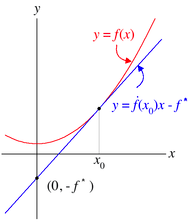
\includegraphics[width=6cm]{./figures/5.png}
\end{figure}
方程(\ref{5.32})是对应于模型A的弱非均匀聚合物溶液的自由能(以$k_BT$为单位)的表达式。在适用平均场近似且密度不均匀性小的情况下是有效的。正如将在第6章讨论的那样,平均场近似适用于模型A,其浓度足够高满足
\begin{equation}
C\gg B\equiv\frac{u_0N^2}{R_g^3}
\end{equation}
其中$C=nR_g^3/V$是在方程(\ref{5.5})中引入的无量纲链浓度,$B$是无量纲消除体积参数。

方程(\ref{5.32})的一个有用的应用是估计聚合物溶液的均相相对于小幅度密度扰动的稳定性。通过检查二次系数可以确定稳定性。
\begin{equation}\label{5.34}
\hat{\Gamma}_2(k)=\frac{1}{\rho_0N\hat{g}_D(k^2R_g^2)}+u_0
\end{equation}
作为波数$k=\left|\bk\right|$的函数。由于$\hat{g}_D(x)$是$x$的单调递减函数,因此,$\hat{\Gamma}_2(k)$的最小值与$k=0$一致。均匀相或螺旋线的稳定极限因此对应于
\begin{equation}\label{5.35}
\hat{\Gamma}_2(0)=\frac{1}{\rho_0N}+u_0=0
\end{equation}
由此得出,在平均场近似中,当$u_0$达到负值$-1/(\rho_0N)$时,模型A呈现出长波长(k=0)不稳定性,这种不稳定性产生宏观相分离:一种富含聚合物;另一种富含溶剂。尽管模型A对于消除体积参数$u_0$的负值定义不明确,但是对应于较差的溶剂条件,平均场螺旋线的极限可以通过方程(\ref{5.35})得出。然而,为了研究在穿过螺旋线边界时出现的新相的性质,我们有必要改用模型B。

RPA展开可用于研究第4章中描述的许多其他模型的均相稳定性。通常,人们获得类似于方程(\ref{5.32})的表达式,即
\begin{equation}\label{5.36}
F[\rho]=F_0+\frac{1}{2V}\sum\limits_{\bk}\hat{\Gamma}_2(k)\widehat{\Delta\rho}(\bk)\widehat{\Delta\rho}(-\bk)+O(\Delta\rho^3)
\end{equation}
但是$\hat{\Gamma}_2(k)$的形式取决于模型。对于模型B,可以得到
\begin{equation}\label{5.37}
\hat{\Gamma}_2(k)=v_0\left(\frac{1}{\phi_{P0}N\hat{g}_D(k^2R_g^2)}+\frac{1}{\phi_{S0}}-2\chi_{PS}\right)
\end{equation}
其中$\phi_{P0}\equiv n_PNv_0/V$是平均聚合物体积分数,$\phi_{S0}=n_Sv_0/V=1-\phi_{P0}$是平均溶剂体积分数,$v_0$是每个聚合物链段的体积和溶剂分子。在模型B中,$\Delta\rho(\br)$可以解释为$\Delta\rho_P(\br)$或$\Delta\rho_S(\br)$,因为它是由于其不可压缩性而导致的,即$\Delta\rho_P(\br)=-\Delta\rho_S(\br)$。对于较小聚合物体积分数,$\phi_{P0}\ll 1$,当我们使$u_0=v_0(1-2\chi_{PS})$对应时,可得到与方程(\ref{5.35})相对应的稳定极限。然而,对于模型B,可以通过假定$\hat{\Gamma}_2(0)=0$获得的液-液相分离的螺旋线边界不同于在更高聚合物浓度下的模型A的螺旋线。实际上,模型B的表达式与熟悉的聚合物溶液的Flory-Huggins晶格理论的螺旋线一致(de Gennes,1979)。

最后一个例子对应于不可压缩的AB两嵌段共聚物熔体。在一篇经典论文(Leibler,1980)中,Leibler得到了模型E密度不均匀的四阶RPA展开,$\Delta\rho\equiv\Delta\rho_A=-\Delta\rho_B$。对于相等的统计分段长度,$b\equiv b_A=b_B$,展开式中的二次系数具有以下形式
\begin{equation}\label{5.38}
\hat{\Gamma}_2(k)=\frac{v_0}{N}\left[\gamma(k^2R_g^2,f)-2\chi_{AB}N\right]
\end{equation}
其中$R_g^2=Nb^2/6$是共聚物的无扰动回旋半径,函数$\gamma(x,f)$由下式定义
\begin{equation}
\gamma(x,f)=\frac{\hat{g}(1,x)}{\hat{g}(f,x)\hat{g}(1-f,x)-(1/4)[\hat{g}(1,x)-\hat{g}(f,x)-\hat{g}(1-f,x)]^2}
\end{equation}
在这个表达式中,$\hat{g}(f,x)$是修正后的Debye函数
\begin{equation}
\hat{g}(f,x)\equiv\frac{2}{x^2}[fx+\exp(-fx)-1]
\end{equation}
在固定嵌段共聚物组成$f$(A嵌段的体积分数)下,函数$\gamma(x,f)$在$x$,$x_m(f)$的非零值处具有依赖于$f$的最小值,由下式给出:
\begin{equation}
\frac{\partial\gamma(x,f)}{\partial x}\bigg|_{x=x_m}=0
\end{equation}
在对称两嵌段共聚物的情况下,$f=1/2$,$x_m(1/2)=3.785$,因此,均相嵌段共聚物熔体中最不稳定的密度形式$\widehat{\Delta\rho_A}(\bk)$具有非零波数$k=[x_m(f)]^{1/2}/R_g$,相应波长$\lambda=2\pi R_g/[x_m(f)]^{1/2}$。这种有限长度尺度不稳定性表示波长接近$\lambda$的周期性中间相的开始。

从$\gamma(x_m,f)-2\chi_{AB}N=0$的关系中得到了共聚物熔体均相分离的稳定极限。这产生了在图5.3中所示的$\chi_{AB}N$对$f$的平面中的曲线,其描述了在平均场近似中均匀两嵌段熔体稳定或不稳定的区域。在$f=1/2$时,我们观察到对称共聚物熔体的稳定极限为$\chi_{AB}N=10.495$。在平均场理论中,在$f=1/2$以外的所有部分中,相与各种有序之间的有序-无序跃迁是一种一级相变,因此需要更高的展开项来精确地区分这两种变化曲线。同时也决定了在通过这个过程时所出现的有序性和对称性(Leibler,1980)。在实践中,这种高阶分析变得非常简单,并且仅限于弱有序的再结晶技术,所谓的弱偏析技术已经发展到了这样一个阶段,即对全平均场方程的直接数值方法,这是5.3节的主题,一般用于研究嵌段共聚物和溶液中的生成。
\begin{figure}[H]
      \centering
      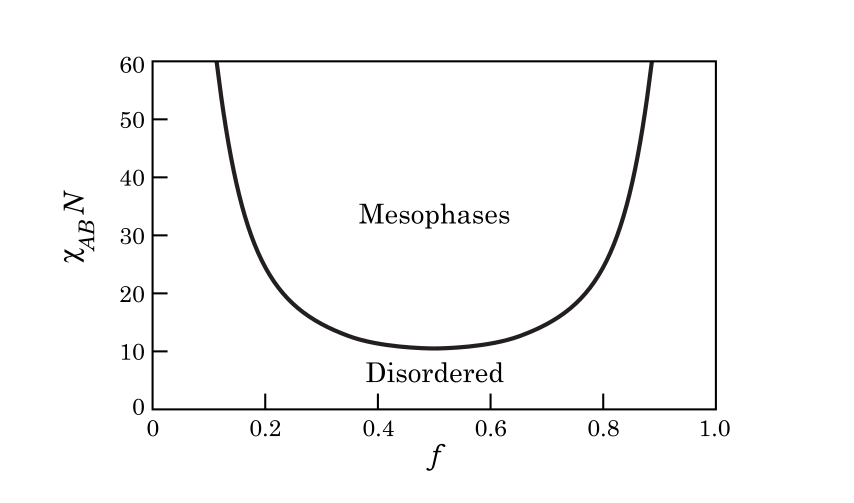
\includegraphics[width=12cm]{./figures/4.png}
      \caption{不可压缩AB两嵌段共聚物熔体的Spinodal曲线由模型E描述。表示为“无序”的区域表示块偏析强度$\chi_{AB}N$和组成$f$的值,对于该组成$f$是均匀的,组成无序相对于小振幅组成扰动是稳定的。表示为“Mesophases”的区域对应于$\chi_{AB}N$和$f$,使得无序相相对于小振幅,有限波长组成扰动不稳定,表明微相分离的开始。在平均场近似中,一阶ODT曲线在接近所示的螺旋线的任何地方,并且两条曲线在$f=1/2$,$\chi_{AB}N=10.495$处合并,其中转变被预测为二阶的。}
\end{figure}
理解聚合物溶液和嵌段共聚物相应的线性特征的物理根源是非常重要的。聚合物溶液为防止不均匀性的,因为存在与组织链相关联的构象熵损失,以支持非均匀的区域段密度分布。从方程(\ref{5.34})可以看出,这种自由能损失随着不均匀性的波数$k$增加,并且随着$k\gg R_g^{-1}$渐进地增长为$k^2$。同样的方法也适用于嵌段共聚物,从大波数$k$可以推断出。然而,嵌段共聚物熔体不能承受任意长波长(小$k$)成分的波动,因为这将需要拉伸单个共聚物链,使$A$段和$B$段在很长的距离内分离。这种拉伸导致了一种熵损失,其根据方程(\ref{5.38})增长为$k^2$当$k\rightarrow 0$。因此,连接每种共聚物的两个嵌段的化学键的集体表现形式是$k_m=\sqrt{x_m}/R_g$,对于共聚物熔体中的组成波动,存在优选的波数。
该优选的波数反应了对共聚物分子量和平均组成构象熵损失,更一般地,对嵌段共聚物结构,尽管由$k_m$设定的长度尺寸与在ODT处形成的周期性中间相的晶格常数相关,但是在进入相图的有序区域时,晶格常数以RPA分析无法预测的方式发展(Almdal,1990;Matsen和Bates,1996b)

RPA展开中的二次系数$\hat{\Gamma}_2(k)$与由下式定义的均匀流体相的结构因子$S(k)$相关联。
\begin{equation}
S(k)=V^{-1}\int\mathrm{d}\br\int e^{-i\bk\cdot(\br-\br')}\left\langle[\hat{\rho}(\br)-\rho_0][\hat{\rho}(\br')-\rho_0]\right\rangle_0\mathrm{d}\br'
\end{equation}
其中下标$0$平均表示没有外场,$J=0$,相互作用系统中的链构象的整体平均值。结构因子与用中子,X射线或光进行的辐射散射实验有关(Hansen和McDonald,1986)。$\Gamma_2(k)$和$S(k)$之间的形式联系是通过应用线性理论建立的,对于模型A来说意味着
\begin{equation}
\left\langle\hat{\rho}(\br)\right\rangle_J=\rho_0-\int\left\langle\hat{\rho}(\br)\hat{\rho}(\br')\right\rangle_0J(\br')\mathrm{d}\br'+O(J^2)
\end{equation}
假设$\int J(\br)\mathrm{d}\br=0$,该公式是通过$J$中的直接扰动展开得出的。表明相应的静态线性函数与没有外场情况下的密度-密度相关函数成比例,即
\begin{equation}\label{5.44}
\frac{\delta\left\langle\hat{\rho}(\br)\right\rangle_J}{\delta J(\br')}\bigg|_{J=0}=-\left\langle\hat{\rho}(\br)\hat{\rho}(\br')\right\rangle_0
\end{equation}
如果我们从密度泛函理论的讨论中引用(4.200),那么得到
\begin{equation}\label{5.45}
\frac{\delta^2F[\left\langle\hat{\rho}\right\rangle_J]}{\delta\left\langle\hat{\rho}(\br)\right\rangle_J\delta\left\langle\hat{\rho}(\br')\right\rangle_J}=-\frac{\delta J(\br)}{\delta\left\langle\hat{\rho}(\br')\right\rangle_J}
\end{equation}
结合方程(\ref{5.44})和(\ref{5.45})得出
\begin{equation}
\frac{\delta^2F[\rho]}{\delta\rho(\br)\delta\rho(\br')}\bigg|_{J=0}=[\left\langle\hat{\rho}(\br)\hat{\rho}(\br')\right\rangle_0]^{-1}
\end{equation}
我们重新使用了简化符号$\rho\equiv\left\langle\hat{\rho}\right\rangle_J$,右端的上标$-1$表示方程(C.29)意义上的函数逆。最后,在傅里叶空间,
\begin{equation}
\frac{\partial^2F[\rho]}{\partial\widehat{\Delta\rho}(\bk)\partial\widehat{\Delta\rho}(-\bk)}\bigg|_{\Delta\rho=0}=\frac{\hat{\Gamma}_2(k)}{V}=\frac{1}{VS(k)}
\end{equation}
它建立了所需的关联$S(k)=1/\hat{\Gamma}_2(k)$。这是无序相波动的一般结果,尽管RPA公式(\ref{5.34}),(\ref{5.37})和(\ref{5.38})依赖于平均场近似。这些表达式在散射实验中都得到了很好的测试(des Cloizeaux和Jannink,1990;Bates和Hartney,1985)。

最后,我们指出平均场近似中出现的不一致性。直接应用方程(4.78)与平均场表达式$\left\langle w(\br)w(\br')\right\rangle\approx w^*(\br)w^*(\br')$导出$S(k)=u_0^{-1}$的无序相模型A,当忽略$w$场波动时无序相无结构的这种明显结果与严格的平均场近似一致。相反,当与方程(\ref{5.34})结合时,上面得到的公式$S(k)=1/\hat{\Gamma}_2(k)$对模型A的无序相中的密度波动做出了不同的陈述,在相互作用场理论的平均场近似中是众所周知的(Amit,1984;Goldenfeld,1992)。在精确计算中,这两种方法必须出现相同的结果,然而,在精确波动公式$S(k)=1/\hat{\Gamma}_2(k)$中使用$\hat{\Gamma}_2(k)$的RPA表达式实际上提供了超出严格的平均场理论并且在高斯水平中包含$w$场波动的结果。这一点将在第6章进一步讨论。
\subsubsection{慢梯度}
可以与平均场近似相结合的另一种有用的近似方案是3.4.2节的慢梯度展开。这里的基本假设是自洽场$w^*(\br)$和相关的分段密度$\left\langle\hat{\rho}(\br)\right\rangle$在长度尺寸上缓慢变化,与聚合物的回旋半径$R_g$相当。同样,我们用模型A说明了这一点,并着重于密度函数$F[\rho]$的构造。如Tang和Freed(1991)所示,巨正则系综证明了开发这种慢梯度展开最方便。

首先巨正则模型类似于平均场表达式(\ref{5.25})为
\begin{equation}
\rho(\br)=\tilde{\rho}_G(\br;[\mu^*])
\end{equation}
我们定义了$\mu^*(\br)\equiv iw^*(r)+J(\br)$并再次使用简写$\rho(\br)$代替$\left\langle\hat{\rho}(\br)\right\rangle$。将此结果与方程(3.157)和(4.76)相结合得到
\begin{equation}\label{5.49}
\rho(\br)=zNe^{-N\mu^*(\br)}\left\{1+R_g^2\left(\frac{N^2}{6}\left|\nabla\mu^*\right|^2-\frac{N}{3}\nabla^2\mu^*\right)+\cdots\right\}
\end{equation}
证明:由$\rho(\br)=\tilde{\rho}_G(\br;[\mu^*])$和$\tilde{\rho}_G(\br;[\mu^*])=zVQ[\mu^*]\rho(\br;[\mu^*])$以及
\begin{equation*}
\rho(\mathbf{x};[W])\sim\frac{\rho_0e^{-W(\mathbf{x})}}{Q[W]}\left\{1+\epsilon_s\left(\frac{1}{6}|\nabla_{\mathbf{x}}W|^2-\frac{1}{3}\nabla_{\mathbf{x}}^2W\right)+\cdots\right\}
\end{equation*}
所以
\begin{equation*}
\rho(\br)=zVQ[\mu^*]\frac{\rho_0e^{-W(\mathbf{x})}}{Q[\mu^*]}\left\{1+\epsilon_s\left(\frac{1}{6}|\nabla_{\mathbf{x}}W|^2-\frac{1}{3}\nabla_{\mathbf{x}}^2W\right)+\cdots\right\}
\end{equation*}
再由$\rho_0=\frac{N}{V}$,$\epsilon_s\rightarrow R_g^2$和$W\rightarrow N\mu^*$得:
\begin{equation*}
\rho(\br)=zNe^{-N\mu^*(\br)}\left\{1+R_g^2\left(\frac{N^2}{6}\left|\nabla\mu^*\right|^2-\frac{N}{3}\nabla^2\mu^*\right)+\cdots\right\}
\end{equation*}
其中被忽略的项是$\mu^*$的梯度的四阶和更高项。方程(\ref{5.49})将$\rho$表示为$\mu^*$的梯度展开。可以反解该函数关系以在$\rho$的梯度中表示$\mu^*$,即
\begin{equation}\label{5.50}
\begin{aligned}
\mu^*(\br)=&-\frac{1}{N}\ln[\rho(\br)/zN]\\
&-\frac{R_g^2}{6N[\rho(\br)]^2}\left|\nabla\rho\right|^2+\frac{R_g^2}{3N\rho(r)}\nabla^2\rho+\cdots
\end{aligned}
\end{equation}
巨正则系综中模型A的平均场方程意味着$iw^*(\br)=u_0\rho(\br)$。因此,通过从等式(\ref{5.50})的两端减去$u_0\rho$来获得$\rho$的梯度中的$J=\mu^*-iw^*=\mu^*-u_0\rho$的展开。

下一步是研究巨正则哈密顿量的展开
\begin{equation}
H_G[w^*,J]=\frac{1}{2u_0}\int[w^*(\br)]^2-zVQ[\mu^*]\mathrm{d}\br
\end{equation}
在$J$的梯度也即在$\rho$的梯度。使用方程(3.156)和方程(\ref{5.50})得到
\begin{equation}\label{5.52}
H_G[w^*,J]=-\int\left(\frac{1}{N}\rho+\frac{u_0}{2}\rho^2-\frac{R_g^2}{3N}\nabla^2\rho+\cdots\right)\mathrm{d}\br
\end{equation}
最后,为了完成计算,我们通过Legendre变换把$J$的泛函变换到$\rho$的泛函
\begin{equation}\label{5.53}
F[\rho]=H_G[w^*,J]-\int J(\br)\rho(\br)\mathrm{d}\br
\end{equation}
将方程(\ref{5.50})和(\ref{5.52})替换为方程(\ref{5.53})得到
\begin{equation}\label{5.54}
F[\rho]=\int\left(\frac{1}{N}\rho\ln\rho+\frac{u_0}{2}\rho^2+\frac{b^2}{36\rho}\left|\nabla\rho\right|^2+\cdots\right)\mathrm{d}\br
\end{equation}
其中$\int\rho(\br)\mathrm{d}\br$中的线性项已被去掉,因为它们可被吸收到参考化学势中。\\
证明:因为
\begin{equation*}
H_G[w^*,J]=-\int\left(\frac{1}{N}\rho+\frac{u_0}{2}\rho^2-\frac{R_g^2}{3N}\nabla^2\rho+\cdots\right)\mathrm{d}\br
\end{equation*}
又
\begin{equation*}
\begin{aligned}
\int J(\br)\rho(\br)\mathrm{d}\br&=\int(\mu^*\rho-u_0\rho^2)\mathrm{d}\br\\
&=\int(-\frac{1}{N}\ln[\rho(\br)/zN]\rho-\frac{R_g^2}{6N\rho(\br)}\left|\nabla\rho\right|^2+\frac{R_g^2}{3N}\nabla^2\rho-u_0\rho^2)\mathrm{d}\br
\end{aligned}
\end{equation*}
所以
\begin{equation*}
\begin{aligned}
F[\rho]&=H_G[w^*,J]-\int J(\br)\rho(\br)\mathrm{d}\br\qquad (R_g^2=\frac{Nb^2}{6})\\
&=\int\left(\frac{1}{N}\rho\ln\rho+\frac{u_0}{2}\rho^2+\frac{b^2}{36\rho}\left|\nabla\rho\right|^2+\cdots\right)\mathrm{d}\br
\end{aligned}
\end{equation*}
方程(\ref{5.54})是众所周知的结果(Tang和Freed,1991),其表示由A型描述的聚合物溶液的自由能(以$k_BT$为单位)作为聚合物链段密度$\rho(\br)$的函数。右端的第一项描述了聚合物的平移熵,而第二项描述了溶剂介导的链段相互作用。第三个“渐变梯度”或“Lifshitz熵”是由密度不均匀产生的构象熵罚因子的长波长近似,方程(\ref{5.54})依赖于平均场近似和慢梯度展开,因此它仅适用于任何地方密度变化满足$\left|\nabla\rho\right|/\rho\ll R_g^{-1}$。与RPA自由能函数方程(\ref{5.32})的一个重要区别是,方程(\ref{5.54})并不局限于振幅较弱但波长较长的不均匀性。在它们都有效的区域,两个表达式重合。例如,将$\rho(\br)=\rho_0+\Delta\rho(\br)$代入方程(\ref{5.54})并且在$\Delta\rho$中展开为二阶的变成方程(\ref{5.36})形式的表达式,但是具有由二次系数给出的二次系数为
\begin{equation}
\hat{\Gamma}_2(k)=\frac{1}{\rho_0N}\left(1+\frac{1}{3}k^2R_g^2+\cdots\right)+u_0
\end{equation}
然而,该等式与PRA展开式(\ref{5.34})至$O(k^2R_g^2)$的小波数$k$(长波长)一致。

\subsubsection{基态优势近似}
3.4.3节中的基态优势近似是一种可以和平均场近似结合使用的非常有效的方法.当高分子聚合物限制在与$R_g$的尺度相比较小的区域上时,这种组合是比较合适的.我们通过回到现在所熟悉的正则系综中模型$A$的自由能问题泛函的推导来引入这个主题.

正则模型$A$中的平均场公式$(5.20)$和$(5.21)$可以简便的表示为:
\begin{equation}
\rho(\mathbf{r}) = \tilde{\rho}(\mathbf{r};[iw^*+J]),\,iw^*(\mathbf{r}) = u_0 \rho(\mathbf{r})
\end{equation}
从而方程$(3.167)$和$(4.75)$可以进一步和基态优势近似结合,得到
\begin{equation}
\rho(\mathbf{r}) = \tilde{\rho}(\mathbf{r};[iw^*+J]) = nN[\Psi(\mathbf{r})]^2
\end{equation}
公式中的基态特征函数$\Psi(\mathbf{r})$满足$w \rightarrow iw^*+J$时的公式$(3.160)$,即
\begin{equation}
\frac{b^2}{6} {\bigtriangledown}^2 \Psi(\mathbf{r}) = [iw^*(\mathbf{r})+J(\mathbf{r})-\Lambda]\Psi(\mathbf{r})
\end{equation}
其中$\Lambda$是基态特征值.从而外场$J$可以表示为
\begin{equation}
J(\mathbf{r}) = \frac{b^2}{6 \Psi(\mathbf{r})} \triangledown^2 \Psi(\mathbf{r}) - u_0 \rho(\mathbf{r}) + \Lambda
\end{equation}
将这个结果代入公式$(4.206)$和$(5.25)$得到下面的密度泛函:
\begin{equation}
F[\rho] = \int (-\frac{nNb^2}{6}\Psi\bigtriangledown^2\Psi+\frac{u_0}{2}\rho^2-\Lambda\rho)\,\mathrm{d}\mathbf{r}
\end{equation}
其中$-n\ln Q[iw^*+J]$项被忽略掉了,因为其比$O(\frac{1}{N})$还要小.

接下来的任务就是将(5.55)式中的$\Psi$替换成$\rho$,重新表示密度泛函.通过对(5.52)式做梯度求导,可得$|\bigtriangledown\Psi|^2 = |\bigtriangledown\rho|^2/(4nN\rho)$,将此式代入(5.55)并做分部积分,可得自由能泛函:
\begin{equation}
F[\rho] = \int (\frac{b^2}{24\rho}|\bigtriangledown\rho|^2+\frac{u_0}{2}\rho^2-\Lambda\rho)\,\mathrm{d}\mathbf{r}
\end{equation}
在上述表达式中保留了与$\Lambda$成比例的项.实际上,$\Lambda$也可以被吸收在拉格朗日乘子(化学势)$\mu$中,$\mu$在(4.202)中用来构造巨势$\Omega(\rho)$并加强限制$\int \rho(\mathbf{r})\,\mathrm{d}\mathbf{r}=nN$.

(5.56)给出的自由能泛函与(3.169)中的泛函$F_2[\rho] = \int (\frac{b^2}{24\rho}|\bigtriangledown\rho |^2+w\rho-\Lambda\rho )\,\mathrm{d}\mathbf{r}$非常相似.实际上,令(3.169)中的$w\rightarrow iw^*/2 = u_0\rho/2$即可得到(5.56)式.从公式我们可以看到非均匀聚合物溶液的自由
能泛函在基态近似可以作为$Lifshitz$熵项和平均场段与段之间相互作用项的和.$Lifshitz$熵反应了与非均匀密度分布$\rho (\mathbf{r})$相关的构象熵惩罚.

公式(5.56)和(5.49)中由慢梯度展开推导的自由能泛函$F[\rho] = \int (\frac{1}{N}\rho\ln\rho+\frac{u_0}{2}\rho^2+\frac{b^2}{36\rho}|\bigtriangledown\rho|^2+\dots)\,\mathrm{d}\mathbf{r}$ 在形式上很相似.在基态近似表达式中,平移熵项$(\frac{\rho}{N})\ln \rho$在$N\rightarrow\infty$或$\frac{\xi}{R_g}\rightarrow0$(其中$\xi $为聚合物位置所在区域的宽度)时消失了,这符合基态近似中要求的$\xi \ll R_g$(即$\rho\rightarrow0$).除此之外,$Lifshitz$熵项的平方梯度系数在公式(5.49)中是$\frac{1}{36}$, 在公式(5.56)中是$\frac{1}{24}$.这种矛盾的起源可以追溯到这样一个事实,在尺度$R_g$上,$\frac{1}{36}$适用于缓慢密度变化,$\frac{1}{24}$则适用于快速密度变化.事实上,我们可以看到对于小振幅密度不均匀性,慢梯度展开(5.49)中的系数$\frac{1}{36}$和$RPA$近似(5.27)对于$kR_g\ll1$时是一致的.相反的,$kR_g \gg 1$时,
(5.56)中的系数$\frac{1}{24}$和$RPA$近似是一致的.换言之,$RPA$和基态优势近似在小振幅上和在$R_g$尺度变换迅速时是保持一致的,然而基态表达式(5.56)并不局限于弱非均匀性展开.

基态优势近似的第二个应用,我们将考虑最初由$Helfand$和$Tagami$解决的对称聚合物与聚合物界面的经典问题.他们研究了一类不可压共聚物混合模型的解析解,这种模型是 具有等统计段长度和聚合度的模型$C$的一种特殊的情况,即$b_A=b_B=b$且$N_A=N_B=N$.这个解依赖于平均场和基态优势近似.其满足如果$\chi_{AB}\ll1$且$N\gg1$,则$\chi_{AB}N\gg1$.强分离极限是指体系由两个在聚合物$A$和$B$中几乎纯的共存相组成,通过一个窄的界面分开,其宽度$\xi$比旋转半径$R_g=b(\frac{N}{6})^2$小得多.

$Helfand$和$Tagami$考虑的情况对应于一个位于$z=0$处的平面界面,将在$z\rightarrow +\infty$的A共聚物的纯相和在$z\rightarrow -\infty$的B共聚物的纯相分开.平均场方程对应于
\begin{equation}
{\frac{\delta H[w_\pm]}{\delta w_+(z)}}|_{w_\pm = w^*_\pm} = i\rho_0[\phi_A(z;[w^*_A])+\phi_B(z;[w^*_B])-1] = 0
\end{equation}
\begin{equation}
{\frac{\delta H[w_\pm]}{\delta w_-(z)}}|_{w_\pm = w^*_\pm} = \rho_0[\frac{2}{\chi_{AB}}w^*_-(z)-\phi_A(z;[w^*_A])+\phi_B(z;[w^*_B])]=0
\end{equation}
其中$w_A=iw_+ - w_-$,$w_B=iw_+ +w_-$为$A$,$B$单体的共轭化学势,且$\Phi_K$是$K$类单体的局部体积分数$(K=A,B)$定义为
\begin{equation}
\Phi_K(\mathbf{r};[w_K]) = \tilde{\rho}_K(\mathbf{r};[w_K])/\rho_0
\end{equation}
上述第一个平均场方程(5.57)式表示了不可压缩条件,即两种物质在每个位置的体积分数之和必须为1.第二个鞍点方程(5.58)表示交换化学势场和$A$类的体积分数有关,在自洽场近似中$w^*_-(z) = \chi_{AB}[\phi_A(z;[w^*_A])-\frac{1}{2}]$.

方程(5.57)和(5.58)都难以处理,因其在鞍点$w^*_\pm(z)$处依赖于体积分数$\Phi_K(\mathbf{r};[w^*_K])$.然而,利用基态优势近似,体积分数可以简化成
\begin{equation}
\Phi_K(\mathbf{r};[w_K]) \approx [\Psi_K(z)]^2
\end{equation}
其中基态特征函数$\Phi_K(z)$满足
\begin{equation}
\frac{b^{2}}{6}\frac{\mathrm{d}^{2}}{\mathrm{d} z^{2}} \Psi_{A}(z)=[iw_+^*(z)-w_-^*(z)-\Lambda_A]\Psi_{A}(z)
\end{equation}
以及
\begin{equation}
\frac{b^{2}}{6}\frac{\mathrm{d}^{2}}{\mathrm{d} z^{2}} \Psi_{B}(z)=[iw_+^*(z)+w_-^*(z)-\Lambda_B]\Psi_{B}(z)
\end{equation}
在这些方程中出现的基态特征值$\Lambda_K$的选择如下所述.我们采用了与公式(3.161)不同的标准特征函数,即$\int {\Psi_K}^2\,\mathrm{d}\mathbf{r}=V{\Psi_K}_0$,其中${\Psi_K}_0$是包含在体系中$K$类聚合物段的平均体积分数.

在适当的边界条件下,在两个共聚相之间可以形成一个单平面界面.特别地,当共存相是纯的时,正如渐进情况$\chi_{AB}N\rightarrow\infty$,则$\Psi_{A}(+\infty)=\Psi_{B}(-\infty)=1$且$\Psi_{A}(-\infty)=\Psi_{B}(+\infty)=0$.下面的梯度条件也适用于$K=A,B$:$\Psi_K'(\pm\infty)=\Psi_K''(\pm\infty)=0$.方程(5.61)和(5.62)是和边界条件是保持一致的,所以必须满足$\Lambda_A=\Lambda_B=\Lambda$且$iw_+(\pm \infty)-\frac{\chi_{AB}}{2}-\Lambda=0$.可以选择一个简单的但任意的压力场$w_+(\pm\infty)=0$,从而$\Lambda=-\frac{\chi_{AB}}{2}$.因此,方程(5.61)和(5.62)变成
\begin{equation}
\frac{b^{2}}{6}\frac{\mathrm{d}^{2}}{\mathrm{d} z^{2}} \Psi_{A}(z)=[iw_+^*(z)+\chi_{AB}\Phi_{B}(z)]\Psi_{A}(z)
\end{equation}
以及
\begin{equation}
\frac{b^{2}}{6}\frac{\mathrm{d}^{2}}{\mathrm{d} z^{2}} \Psi_{B}(z)=[iw_+^*(z)+\chi_{AB}\Phi_{A}(z)]\Psi_{B}(z)
\end{equation}
从而,$A$聚合物段受到的平均势场是"压力"项$iw_+^*(z)$和$B$段局部接触相互作用项$\chi_{AB}\Psi_{B}$之和.同样地,$B$聚合物也受到相同的"压力"场,但是相互作用势$\chi_{AB}\Psi_{A}$与$A$段的局部体积分数成比例.

$Helfand$和$Tagami$证明了当$K=A,B$时,由(5.57),(5.60),(5.63),(5.64)五个方程组成的方程组对上述平面边界条件具有解析解,这个解对应于
\begin{equation}
\Psi_{A}(z)=1-\Psi_{B}(z)=\frac{1}{1+e^{\frac{-z}{\xi}}}
\end{equation}
\begin{equation}
\Psi_K(z) = [\Psi_K(z)]^{\frac{1}{2}}
\end{equation}
以及
\begin{equation}
iw_+^*(z)=-3\chi_{AB}\Psi_{A}(z)\Psi_{B}(z)
\end{equation}
其中$\xi$是界面宽度大小,定义为
\begin{equation}
\xi = \frac{b}{2(6\chi_{AB})^{\frac{1}{2}}}
\end{equation}
\begin{figure}[H]
	\centering
	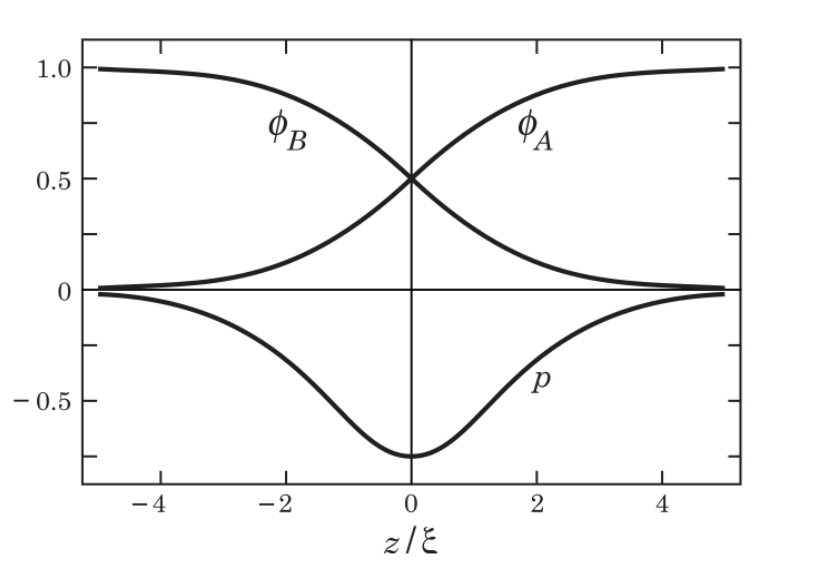
\includegraphics[width=12cm]{./figures/fig5-4.png}
	\caption{对称聚合物-聚合物界面的界面曲线的$Helfand−Tagami$解.$A,B$聚合物段的体积分数分别标记了$\Psi_{A},\Psi_{B}$.整段的体积分数是单位1.$p$曲线表示压力场$p(z)=\frac{iw_+^*(z)}{\chi_{AB}}$.}
\end{figure}

与$Helfand−Tagami$解有关的平衡体积分数曲线$\Psi_{A}(z)$和$\Psi_{B}(z)$如上图所示.界面宽度$\xi$与$A,B$混合区域宽度有关.混合区域宽度与由$\chi_{AB}$参数化的$A−B$接触能相反,与扩散界面提供的构象熵成正比.压力场$iw_+^*(z)$是负的且位于界面区域.场的作用将聚合物吸引到界面上,从而在所有位置看来都是均匀的段密度.

在3.4.3节中基态优势近似的有效性依赖于局部化学势域,其远远小于$R_g$,在本例中局部势就是压力场$iw_+^*(z)$,其约束的不是整条链而是形成界面链段的环.压力场的范围和界面宽度$\xi$是同阶的,这个范围满足规则$\frac{\xi}{R_g} =\frac{1}{2(\chi_{AB}N)^{\frac{1}{2}}}\ll1$,从而$\chi_{AB}N\gg1$.同样地,平均场近似的有效性要求$C\gg1$,其中$C$为公式(5.5)定义的配位数.因为在熔融状态下$C\sim\rho_0b^3N^{\frac{1}{2}}$,所以只要$A$和$B$都是高分子量的,这个条件就满足了,即$N\gg1$.最后,为使$Helfand−Tagami$解是有效的,界面宽度$\xi $必须不能低于介观尺度.换言之,必须有$\xi \gg b$,或等价地,$\chi_{AB}\ll1$.因此,只要满足$\chi_{AB}\ll1$,$N\gg1$以及$\chi_{AB}N\gg1$,就可以确保$Helfand−Tagami$解是有效的.
	
非常重要的是我们要注意到公式(5.68)描述的的是固有的界面宽度,在流体-流体界面实验中测量了非固有界面宽度,它包含了界面的长波长表面波动张力,因此超出了固有界面宽度.这样的表面波动张力可以被看作是一种特殊的场波动,尤其是对于层几何.

对称聚合物-聚合物界面的表面张力可以由$Helfand−Tagami$解获得,注意到张力是每单位表面面积多余的自由能,且在平均场近似中,$A(n_A,n_B,V,T)\approx k_BTH[w_+^*,w_-^*]$.由公式(4.98),界面张力$\gamma$定义如下($Helfand−Tagami$,1971):
\begin{equation}
\begin{aligned}
\gamma&=k_B T \rho_0\int_{-\infty}^{+\infty}(\frac{1}{\chi_{AB}}[w_-^*(z)]^2-iw_+^*(z)-\frac{1}{4}\chi_{AB})\,\mathrm{d}z\\
&=-k_B T \rho_0\int_{-\infty}^{+\infty}(\chi_{AB}\Psi_{A}(z)\Psi_{B}(z)+iw_+^*(z))\,\mathrm{d}z\\
&=2k_B T \rho_0\chi_{AB}\int_{-\infty}^{+\infty}\Psi_{A}(z)\Psi_{B}(z)\,\mathrm{d}z\\
&=k_B T b \rho_0(\frac{\chi_{AB}}{6})^{\frac{1}{2}}
\end{aligned}
\end{equation}
因此强分离聚合物-聚合物界面的表面张力是与聚合物分子量无关的,它的尺度是$Flory$相互作用参数$\chi_{AB}$的平方根.

一个简单的缩放参数可以用来更好的理解公式(5.68),(5.69).正如下图所示,界面区域可以看作是相互混合的环的区域的宽度.界面宽度$\xi$可以表示环路相互混合的区域的宽度.考虑一个典型的包含$g$统计段的环,$g$的值可以看作是均分估计,即:一个环表示一条链对不同聚合物相的相互渗透,这种渗透只在能量损耗为$O(k_B T)$的情况下才能发生.带有$g$个段的环的能量损耗$\sim g\chi_{AB}k_BT$,因此我们可以得出结论$g\sim \frac{1}{\chi_{AB}}$,其在$\chi_{AB} \ll1$时是一个很大的数.因为作用在每个环上的强作用力只与弱热能尺度有关系,界面宽度可以估计成一个未受干扰的$g$段聚合物的大小,即$\xi \sim bg^{\frac{1}{2}}\sim \frac{b}{\chi_{AB}^{\frac{1}{2}}}$.这个尺度很显然是与公式(5.68)是保持一致的.最后,界面张力可以估计成由$A−B$接触引起的界面多余自由能密度($k_B T\rho_0\chi_{AB}$)乘以区域宽度($\xi$),即得到公式$\gamma\sim k_B T\rho_0b\chi_{AB}^{\frac{1}{2}}$.这个结果很显然是与公式(5.69)是保持一致的.
\begin{figure}[H]
	\centering
	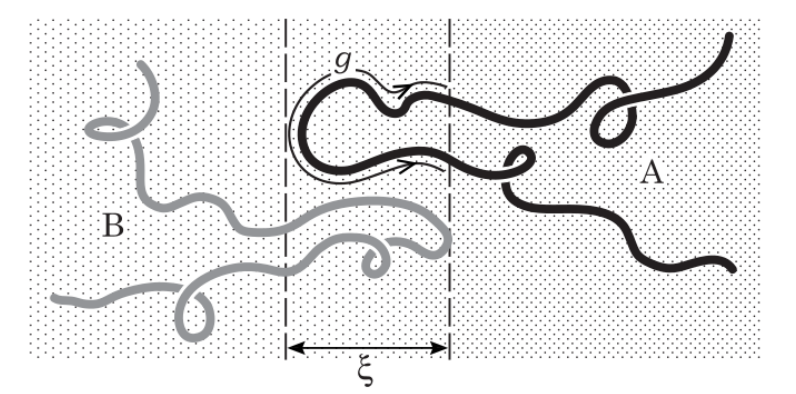
\includegraphics[width=12cm]{./figures/fig5-5.png}
	\caption{聚合物-聚合物界面的链构象示意图.一条穿过界面的聚合物链贡献了带有$g$段的环,且$A$环和$B$环混合穿过宽度为$\xi$的区域.}
\end{figure}

\subsubsection{强拉伸近似}
另一个重要的分析方法是3.4.4.2节中介绍的强拉伸(经典)近似与平均场近似的组合.阐释这种方法的一个有用的背景就是用模型$K$描述的溶液聚合物刷.在足够高的密度
系链下,刷中的聚合物被强烈拉伸,可以采用这种经典的近似.

在平均场近似中,(实数)势$\mu(z) = iw^*(z)$和平均段密度$\rho(z) = \tilde{\rho}(z;[iw^*])$在刷中每一个位置处成立以下关系
\begin{equation}
\mu(z) = u_0\rho(z)
\end{equation}
其中采用的是图4.7中的坐标体系.经典路径$z(s)$开始于嫁接面$z(0)=0$,终止于$z(N)=z_0$,且满足公式(3.194),即
\begin{equation}
\frac{3}{b^2}\frac{\mathrm{d}^2}{\mathrm{d} s^2}z(s) = \frac{\mathrm{d}\mu(z(s))}{\mathrm{d}z(s)}
\end{equation}
因为不管末端位置是什么,刷中所有的链都具有$N$个统计段,"等时间限制"($Milner\,et\,al.,1988$)说明$\mu(z)$经典的近似必须是调和势,即$\mu(z) = C_1-C_2 z^2$.带有这样的调和势,并带有条件$z(0)=0$,$z(N)=z_0$且$[\frac{\mathrm{d}z(s)}{\mathrm{d}s}]_{s=N} = 0$(在自由链端没有张力),方程(5.71)中的经典路径可以求解出来:
\begin{equation}
z(s) = z_0 \sin(\frac{\pi s}{2N})
\end{equation}
平方项系数
\begin{equation}
C_2 = \frac{3\pi^2}{8b^2N^2}
\end{equation}
第二个系数$C_1$可以由段关系定义:
\begin{equation}
\sigma N = \int_{0}^{h}\rho(z)\,\mathrm{d}z = (u_0)^{-1}\int_{0}^{h}(C_1-C_2 z^2)\,\mathrm{d}z
\end{equation}
其中$h=(\frac{C_1}{C_2})^{\frac{1}{2}}$是聚合物刷厚度,有定义$\rho(h)=0$.公式(5.74)相当于
\begin{equation}
C_1 = \frac{\sigma u_0 N}{h}+\frac{C_2 h^2}{3}
\end{equation}
通过组合这些结果,我们得到了一个关于平衡刷厚度的重要公式($Milner\,et\,al.,1988$)
\begin{equation}
h = (\frac{4}{\pi^2})^{\frac{1}{3}}(\sigma u_0)^{\frac{1}{3}}b^{\frac{2}{3}}N
\end{equation}

这公式有效的一个标准是聚合物被拉伸到一个高度,其远远超过了它们未受干扰的尺度,$\frac{h}{R_g}\gg 1$,相当于$(\frac{\sigma u_0}{b})^{\frac{1}{3}}N^{\frac{1}{2}}\gg 1$,或者等价于$(\sigma {R_g}^2)B\gg 1$,其中$B$是由(5.28)定义的无量纲体积分数参数.我们将可以看到参数$B$将在第六章中,在聚合物溶液中评估排除体积效应的强度起到一个重要的作用.

在平均场密度近似和强拉伸近似的组合中,平衡段密度曲线$(u_0/C_1)\rho (z) = 1-(\frac{z}{h})^2$在下图中画了出来.这个抛物曲线反应了在高嫁接密度时平均场段密度分布.然而,图中的虚线显示,强拉伸近似对平均场曲线的近似并不是一致有效的,在表面和刷的外边界周围都是由偏差的.在$z=0$附近的耗长边界层已经在4.9.4节中讨论过了.
事实上,带有适用于在$z=0$的传播子的$Dirichlet$条件的模型$K$的全平均场的解显示了一个尖锐层,正如下图的虚线所示.密度梯度随着嫁接的密度$\sigma$的增大而增大.从图中我们可以清晰地看到,强拉伸近似只适用于边界层外,其中$\mu(z)$缓慢变化,且在$z=0$处符合黎曼边界条件.同样地,在刷的外边界,平均场方程的近似解表现了密度曲线的缓慢变化,与突然终止于$z=h$的抛物曲线相反.外边界层是由于在刷子边缘的强烈拉伸引起的,这个区域$h$中,平均密度曲线是多个聚合物构象的结果.$Matsen$对于"干聚合物刷"的强拉伸近似和平均场近似之间,以及在干刷和化学性质相同的均聚物熔体之间的界面做了相似的比较.
\begin{figure}[H]
	\centering
	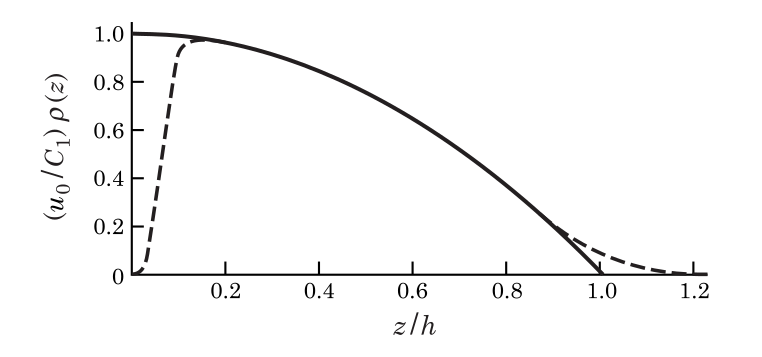
\includegraphics[width=12cm]{./figures/fig5-6.png}
	\caption{聚合物刷的模型$K$的平均场近似和强拉伸近似组合得到的段密度曲线$\rho(z)$的示意图.在高嫁接密度下,实曲线表示全平均场密度分布,边界层如虚线所
		示.在表面附近,经典近似采用黎曼边界条件且忽略了狭窄的耗尽层.在刷的外边界,强拉伸近似衰弱下来形成了一条光滑的曲线.}
\end{figure}

模型$K$的强拉伸理论和全平均场解都忽略了$w$场波动.在嫁接点$\sim \sigma^{-\frac{1}{2}}$,当短波长低于平均间距的情况下,场波动是最强烈的,且引起了刷的不能在平均场近似中看到的一个局部的排除体积效应.排除体积效应可以通过利用"斑点事件"近似地纳入平均场理论中,但是完全处理需要通过第六章中的数值方法.和本节相关的,我们将注意到经典近似中的已经被$Semenov$证明的一个有力的静电类比.这个类比已经被证实对非均匀聚合物的各种计算是非常有效的,其中强链拉伸的假设是合理的.

